\documentclass[compress,11pt]{beamer}
%\includeonly{pendel}
\usetheme{Ilmenau}
%\usetheme{fau-4-3}
%\usecolortheme{beaver}
\beamertemplatenavigationsymbolsempty
\usepackage[ngerman]{babel}
\usepackage{marvosym}
\usepackage{multimedia}
\usepackage[utf8]{inputenc}
\usepackage{amsmath}
\usepackage{amsfonts}
\usepackage{amssymb}
\usepackage{graphicx}
\usepackage{esvect}
%\author{}
\title{EP Gruppe 8}
%\setbeamercovered{transparent}
%\setbeamertemplate{navigation symbols}{}
%\logo{}
%\institute{}
%\date{}
%\subject{}
\usepackage{verbatim}
\begin{document}

\section{Aufgabe 1}
\begin{frame}

\end{frame}


\section{Aufgabe 2}
\begin{frame}
%\includegraphics schaltung
%\end{frame}
%\begin{frame}
\subsection{Erste Version der Schaltung}
\begin{itemize}
\item Transistor hier als Schalter, da Strom nur fließt, wenn $U_{CE} \neq 0$
\item Sobald der Schalter in der ersten Schaltung geschlossen ist, liegt an Collector und Emitter eine Spannung an und der Transistor lässt durch $\Rightarrow$ iode leuchtet
\end{itemize}
\subsection{Zweite Version der Schaltung}
\begin{itemize}
\item Jetzt liegt konstante Spannung an Collektor und Emitter $\Rightarrow$ Transistor sperrt nicht und Diode leuchtet
\item Schaltung
\end{itemize}
\end{frame}













\section{Aufgabe 3}
\subsection{Common-Emitter}
\begin{frame}
Schaltbild:\\
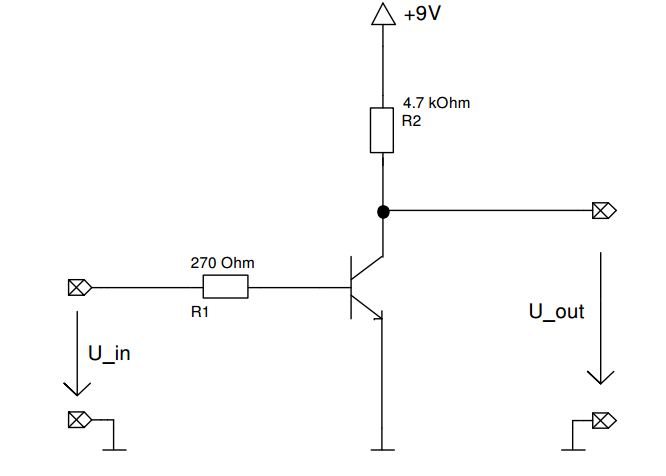
\includegraphics[width=.7\textwidth]{schaltbilder/schalt_3a}\\
Durchfführung:\\ Schaltung wird bei $U_{in}$ mit einer 1kHz-Spannung betrieben, die Amplitude beträgt 1.2 V. Gemessen wird $U_{CE}$
\end{frame}
\begin{frame}
\begin{block}{Funktionsweise der Schaltung}

\begin{itemize}
\item Bei positiver Eingangsspannung $> 0.7 V$ leitet die Basis-Emitter-Strecke des Transistors
\item Je größer die Eingangsspannung, desto größer ist $I_{BE}$ $\Rightarrow$ $U_{CE}$, die abgegriffen wird, wird dementsprechend kleiner $\Rightarrow$ Schaltung invertiert für Positive $U_{in}$
\item Sobald $U_{BE} < 0.7 V$ $\Rightarrow$ Transistor sperrt und Ausgangssignal entspricht den $9 V$ der Gleichspannung
\item Basiswiderstand $R_1$ bestimmt Arbeitspunkt der Schaltung und kann zu dessen Regulierung verwendet werden
\end{itemize}
\end{block}
\end{frame}

\begin{frame}

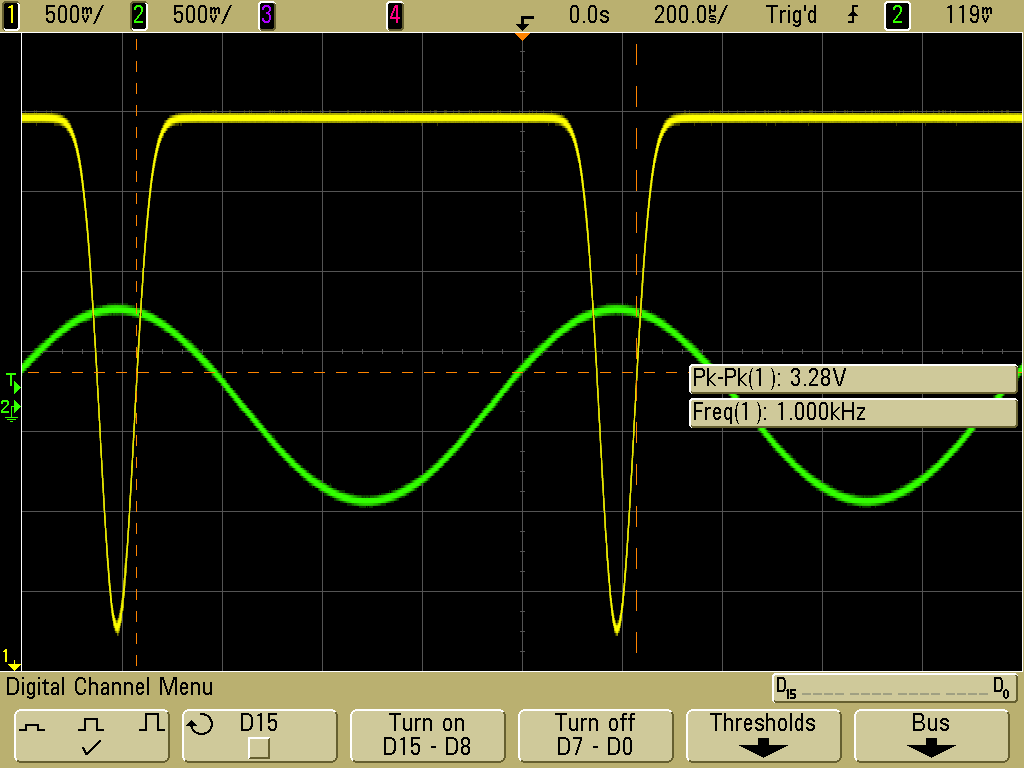
\includegraphics[width=.7\textwidth]{../daten/oszi/scope_45}\\
Beobachtung:\\
Gemessene Amplitude bei Sinusbergen der Eingangsspannung: $U_{out} = 3.28 V$\\
Sonst: $U_{out} = 9 V$
\end{frame}
\begin{frame}
Berechnung der Verstärkung:\\
Nach Vorlesung folgt:
\begin{equation}
U_{out} = U_{cc} - h_{FE} \cdot \frac{R_C}{R_B} \cdot (U_{in} - U_{BE}) \Rightarrow h_{FE} = \frac{(U_{cc} - U_{out})}{(U_{in} - U_{BE}) \cdot \frac{R_C}{R_B}}
\end{equation}
Einsetzen ergibt, da $U_{in,max} = \frac{U_{pp}}{2} = 0.6 V$ und $U_{BE} = 0.7 V$ (Konstante für Dioden) einen negativen, betragsmäßig großen Wert $\Rightarrow$ $U_{BE}$ muss effektiv kleiner sein als $0.7 V$\\
\end{frame}
\begin{frame}

Taktik:
\begin{itemize}
\item projeziere das Intervall, in dem $U_{out} \neq 9 V$ auf das Eingangssignal (nur bei diesen Spannungen ist $U_{in}$ größer als die Durchlassspannung)
\item lese dort die Differenz von maximalen Amplitude zu Funktionswert ab
\end{itemize}


\end{frame}
\begin{frame}
Ablesen ergibt für $\bigtriangleup t_{peak,out} = 200 \mu s$ : $\bigtriangleup U = (U_{in} - U_{BE}) \leq 1 mV$ \\ Für die Verstärkung ergibt sich mit $0.1 V$ also:
\begin{equation}
h_{FE} = \dots 	= 3.28
\end{equation}
Und für den Gain:
\begin{equation}
G = -h_{FE} \cdot \frac{R_C}{R_B} = 57.2
\end{equation}
\end{frame}
\begin{frame}
\begin{block}{Verhalten unter Erwärmung}
\begin{itemize}
\item Bei Berührung mit dem Finger nur leichter, nicht nennenswerter Anstieg der Amplitude
\item Effektiver ist das Hinhalten eines Lötkolben ($T \approx 150 ^{\circ} C$) in die Nähe des Transistors  $\Rightarrow$ Amplitude steigt auf bis zu $7.3 V$ an
\end{itemize}
Grund: Leitfähigkeit des Halbleiters verstärkt sich bei höheren Temperaturen
\end{block}
\end{frame}
\begin{frame}
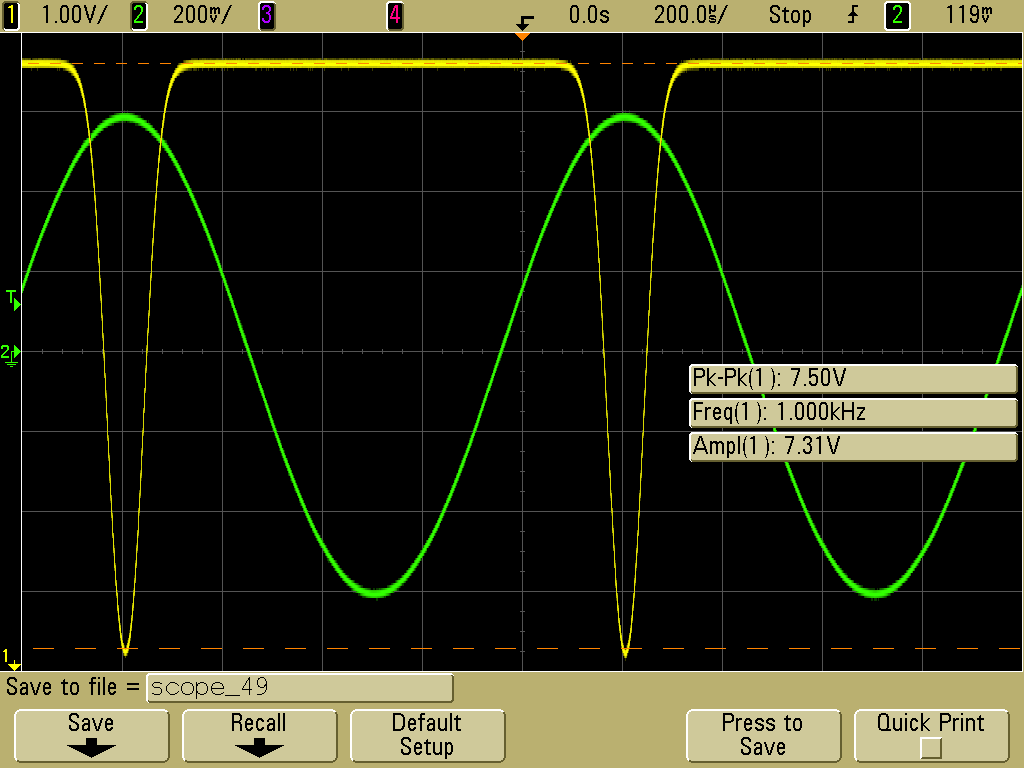
\includegraphics[width=.7\textwidth]{../daten/oszi/scope_49}
\end{frame}
\begin{frame}
Eigenschaften der Schaltung:\\
\begin{itemize}
\item Nicht Linear
\item Spannungen unter $\approx 0.5 V$ werden abgeschnitten $\Rightarrow$ DC-Offset in Spannung nötig, um Signal nur zu verstärken und nicht zu verändern
\item Arbeitspunktbereich im Verstärkungsbereich, wenn Basis öffnet
\end{itemize}
\end{frame}
\subsection{Common-Emitter (verbessert)}
\begin{frame}
Schaltbild:\\
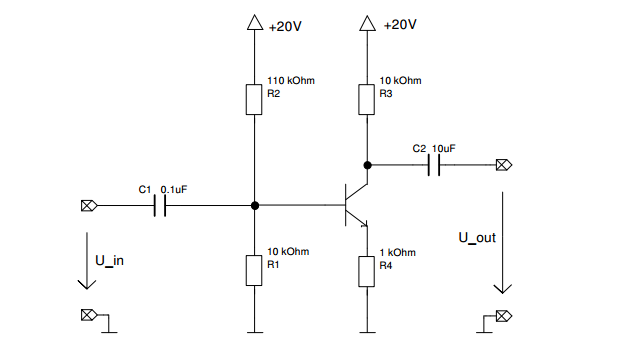
\includegraphics[width=.7\textwidth]{schaltbilder/schalt_3b}\\
Durchführung:\\

Schaltung wurde einmal mit Sinusspannung $U_{in,amp} = 1.25 V$ betrieben, Ausgangssignal wurde invertiert mit $U_{out,amp} = 11.3 V$

\end{frame}
\begin{frame}
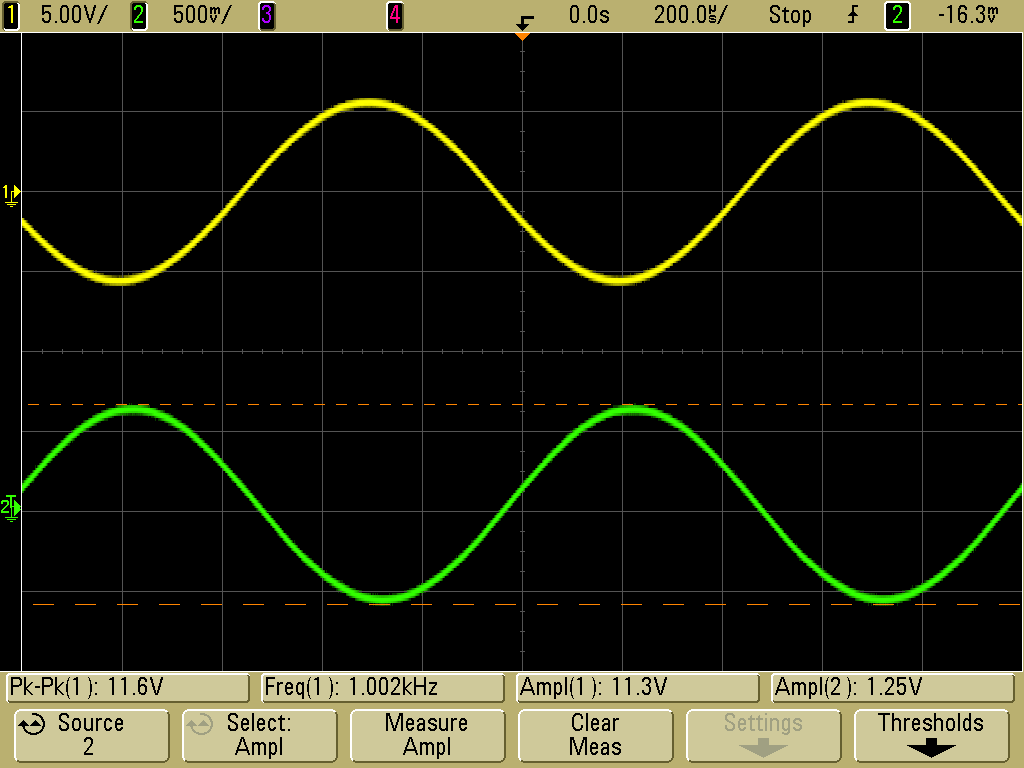
\includegraphics[width=.7\textwidth]{../daten/oszi/scope_51}
\end{frame}
\end{document}
